\subsection{premi/client/navbar}
\begin{figure}[H]
\begin{center}
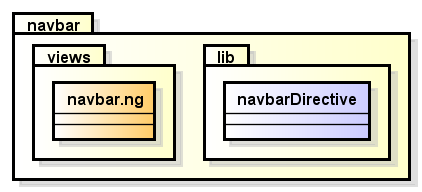
\includegraphics[scale=0.70]{img/diapkg/navbar.png}
\caption{Diagramma della classe premi/client/navbar}
\end{center}
\end{figure}

%-------  diagramma di un template %
\subsubsection{premi/client/navbar/views/navbar.ng}

\begin{description}
%-------  descrizione del template%
\item[Descrizione] \hfill
	template della vista associato alla direttiva \textit{navbarDirective} che permette di inserire la navbar visualizzando l'utente loggato, i bottoni per le impostazioni e l'uscita dalla pagina in cui si trova l'utente in quel momento 
\end{description}

%-------  diagramma di un template %
\subsubsection{premi/client/navbar/lib/navbarDirective}

\begin{description}
%-------  descrizione del template%
\item[Descrizione] \hfill
	direttiva che include la vista \textit{navbar.ng} e permette con il tag html$_G$ \textit{navbar} di visualizzare la navbar
\end{description}